\documentclass[conference,compsoc,final,a4paper]{IEEEtran}
\usepackage[utf8]{inputenx}
\usepackage{amsfonts}

%% Bitte legen Sie hier den Titel und den Autor der Arbeit fest
\newcommand{\autoren}[0]{Arns, Jonathan}
\newcommand{\dokumententitel}[0]{Performance moderner SAT Solver in Theorie und Praxis}

\input{preambel} % Weitere Einstellungen aus einer anderen Datei lesen

\begin{document}

% Titel des Dokuments
\title{\dokumententitel}

% Namen der Autoren
\author{
  \IEEEauthorblockN{\autoren}
  \IEEEauthorblockA{
    Hochschule Mannheim\\
    Fakultät für Informatik\\
    Paul-Wittsack-Str. 10,
    68163 Mannheim
    }
}

% Titel erzeugen
\maketitle
\thispagestyle{plain}
\pagestyle{plain}

% Eigentliches Dokument beginnt hier
% ----------------------------------------------------------------------------------------------------------

% Kurze Zusammenfassung des Dokuments
\begin{abstract}
SAT ist das Problem, ob eine aussagenlogische Formel erfüllbar ist oder nicht. Da SAT $\mathcal{NP}$-vollständig ist, sind effiziente Algorithmen für SAT gleichzeitig für viele andere schwere Probleme anwendbar und sind damit von praktischer Relevanz. Dieser Artikel fasst den aktuellen Erkenntnisstand über die Eigenschaften und die Performance moderner SAT Solver zusammen und argumentiert, dass SAT Solver seit 1992 algorithmisch einen größeren Performancezuwachs hatten, als die Computer Hardware, auf der sie laufen. Abschließend wird ein kurzer Überblick über praktische Anwendungsbereiche moderner SAT Solver, wie formale Verifikation von Hardware und Software Systemen, gegeben.
\end{abstract}

% Inhaltsverzeichnis
{\small\tableofcontents}

\section{Einleitung}
Entwicklung moderner Computer Hardware ist kaum noch ohne formale Verifikation denkbar. Die SAT Solver, die das heute ermöglichen, waren jedoch nicht immer schnell für derartige Anwendungen. SAT Solver selbst sind seit den 90er Jahren bis heute ein ständiges Forschungsthema und haben sich in dieser Zeit viel verändert. \cite{sat_solving_in_practice_2008}

Mit dem näher rückenden Ende des Mooreschen Gesetzes \cite{50_years_of_moore} gewinnen algorithmische Verbesserungen von Software weiter an Bedeutung.
Dieser Artikel stellt deshalb die Frage, ob SAT Solver sich wirklich erheblich weiter entwickelt haben oder ob sie wie viele andere Programme auch hauptsächlich vom Performancezuwachs durch schnellere Hardware profitieren. Dazu werden zuerst die theoretischen Grundlagen gelegt und es wird betrachtet, was einen modernen SAT Solver ausmacht. Zuletzt soll ein Einblick in die praktischen Einsatzmöglichkeiten moderner SAT Solver gegeben werden.

\section{Grundlagen}
Im Folgenden werden die theoretischen Grundlagen für den weiteren Inhalt dieses Artikels gelegt.

\subsection{Turingmaschinen}
Eine Turingmaschine ist ein theoretisches Rechnermodell, das informell aus einem unendlich langen Band-Speicher, einem Lese- und Schreibkopf und einem Steuerwerk, das das Programm enthält und den Lese- und Schreibkopf steuert, besteht. Der Lese- und Schreibkopf kann Zeichen auf dem Band lesen und schreiben und sich um eine Position nach rechts oder links bewegen. Formal wird eine Turingmaschine als 7-Tupel, $(Q, \Sigma, \Gamma, \delta, q_{0}, q_{accept}, q_{reject})$, definiert, wobei $Q, \Sigma, \Gamma$ endliche Mengen sind und
\begin{itemize}
  \item $Q$ die Menge der Zuständen ist,
  \item $\Sigma$ das Eingabealphabet ohne das leere Symbol $\sqcup$ ist,
  \item $\Gamma$ das Bandalphabet ist, mit $\sqcup \in \Gamma$ und $\Sigma \subset \Gamma$,
  \item $\delta: Q \times \Gamma \longrightarrow Q \times \Gamma \times \{L,R\}$ die Übergangs-funktion ist,
  \item $q_{0} \in Q$ der Startzustand ist,
  \item $q_{accept} \in Q$ der akzeptierende Zustand ist und
  \item $q_{reject} \in Q$ der ablehnende Zustand ist.
\end{itemize}
Die Übergangsfunktion $\delta$ definiert die Aktionen der Turingmaschine. Sei die Maschine in einem Zustand $q$, der Lese- und Schreibkopf über einem Bandfeld mit einem Symbol $a$ und $\delta(q,a) = (r,b,R)$, dann schreibt die Maschine das Symbol $b$ an Stelle des Symbols $a$, geht in den Zustand $r$ über und bewegt den Kopf nach rechts. Wäre $\delta(q,a) = (r,b,L)$, würde die Maschine den Kopf nach links bewegen, es sei denn der Kopf befindet sich am Anfang des Bands, dann bewegt sich der Kopf nicht. 
Eine Turingmaschine $M = (Q, \Sigma, \Gamma, \delta, q_{0}, q_{accept}, q_{reject})$ erhält eine Eingabe $w = w_1 w_2 ... w_n \in \Sigma^*$, die ganz links am Anfang des Band-Speichers anfängt. Der Rest des Bands ist mit dem leeren Symbol gefüllt. Der Lese- und Schreibkopf beginnt am Anfang des Bands und $M$ befindet sich zu Anfang im Zustand $q_0$. Die Berechnung folgt den Regeln der Übergangsfunktion $\delta$, bis $M$ in einen der Zustände $q_{accept}$ und $q_{reject}$ übergeht und damit die Eingabe akzeptiert oder ablehnt. Falls $M$ niemals in einen der beiden Zustände kommt, läuft $M$ für immer und produziert kein Ergebnis. \cite{theory_of_computing}

Die Menge von Eingaben, die $M$ akzeptiert, ist die Sprache, die von $M$ erkannt wird. Eine formale Sprache $L$ heißt entscheidbar, wenn es eine Turingmaschine gibt, die jede Eingabe in $L$ akzeptiert und jede andere Eingabe ablehnt, also immer terminiert. Der Begriff der formalen Sprache dient dabei als mathematisches Modell eines Entscheidungsproblems \cite{handbook_theoretical_computer_science}. Nicht jede Sprache ist entscheidbar, es gibt also Probleme, die nicht mit einer Turingmaschine gelöst werden können. \cite{theory_of_computing}

Die Church-Turing These besagt, dass für jeden Algorithmus eine äquivalente Turingmaschine existiert.
Der Begriff des Algorithmus, der informell als eine Reihe von Anweisungen mit dem Ziel eine bestimmte Aufgabe zu lösen definierbar ist, lässt sich damit formal als jede Abfolge von Schritten, die durch eine Turingmaschine abgebildet werden kann, definieren. Damit existiert für jedes mögliche Computer Programm eine äquivalente Turingmaschine. Turingmaschinen bilden also eine theoretische Grundlage für die Grenzen und Möglichkeiten von Computern. Sie dienen als Werkzeug bei der Frage nach der Berechenbarkeit von Problemen. \cite{theory_of_computing} 

\subsection{Nichtdeterministische Turingmaschinen}
Die bis hierher beschriebene Turingmaschine trifft ihre Entscheidungen deterministisch. Eine andere Variante ist die nichtdeterministische Turingmaschine, die sich durch das Gegenteil auszeichnet. Formal ist der einzige Unterschied zu einer deterministischen Turingmaschine die Übergangsfunktion, die stattdessen als $\delta: Q \times \Gamma \longrightarrow \mathcal{P}(Q \times \Gamma \times \{L,R\})$ definiert wird \cite{theory_of_computing}. Informell bedeutet dies, dass es für jede Kombination aus einem Zustand $q$ und einem gelesenen Symbol $a$ mehrere mögliche Übergänge gibt. Die Berechnung einer nichtdeterministischen Turingmaschine ist also ein Baum, dessen Zweige den möglichen Übergängen entsprechen. Die Maschine akzeptiert die Eingabe, wenn ein Zweig den Zustand $q_{accept}$ erreicht. \cite{handbook_theoretical_computer_science}
Für jede nichtdeterministische Turingmaschine existiert eine äquivalente deterministische Turingmaschine, die deren Verhalten in exponentieller Zeit simuliert. Im Gegensatz zu deterministischen Turingmaschinen ist das Verhalten von nichtdeterministischen Turingmaschinen allerdings nicht in realen Computern umzusetzen. \cite{theory_of_computing}

\subsection{Komplexitätsklassen}
Selbst wenn ein Problem grundsätzlich durch eine Turingmaschine und damit einen Computer gelöst werden kann, ist das in der Praxis nicht immer praktikabel, da Probleme grundlegend unterschiedlich komplex sind. Komplexität beschreibt die Zeit und die Menge an Speicher, die zur Lösungs eines Problems nötig sind. In diesem Artikel wird ausschließlich Zeitkomplexität betrachtet und im Folgenden einfach als Komplexität bezeichnet.
Sei $M$ eine deterministische Turingmaschine, dann ist die Komplexität von $M$ die Funktion $f(n)$, wobei $n$ die Länge der Eingabe ist und $f(n)$ die maximale Anzahl der Schritte, die $M$ durchführt, bevor sie mit dem korrekten Ergebnis terminiert. Probleme werden anhand der Komplexität ihrer besten Lösung in unterschiedliche Komplexitätsklassen wie $\mathcal{P}$ und $\mathcal{NP}$ eingeteilt. \cite{theory_of_computing}

$\mathcal{P}$ ist die Klasse der Sprachen, die in polynomieller Zeit durch eine deterministische Turingmaschine entscheidbar sind \cite{handbook_theoretical_computer_science}. Für Turingmaschinen, die ein Problem in $\mathcal{P}$ lösen, ist also die Komplexität $f(n)$ immer ein Polynom wie $f(n) = n^2 + 3n$. Probleme in $\mathcal{P}$ sind in der Regel praktikabel durch einen Computer lösbar, beispielsweise liegt das Sortieren von beliebigen, miteinander vergleichbaren, Objekten in $\mathcal{P}$ \cite{theory_of_computing}.

$\mathcal{NP}$ ist die Klasse der Sprachen, die in polynomieller Zeit durch eine nichtdeterministische Turingmaschine entscheidbar sind \cite{handbook_theoretical_computer_science}. Die beste deterministische Methode um Probleme in $\mathcal{NP}$ zu lösen benötigt allerdings exponentielle Zeit \cite{theory_of_computing}. Da in der Praxis keine nichtdeterministischen Computer existieren, ist die Komplexität der Algorithmen $f(n)$ für viele Probleme in $\mathcal{NP}$ exponentiell, wie $f(n) = 2^n$. $\mathcal{NP}$ ist eine Obermenge von $\mathcal{P}$ \cite{handbook_theoretical_computer_science}.

Probleme lassen sich in andere Probleme übersetzen, so dass die Lösung des Ursprünglichen Problems mit einem Algorithmus für das andere Problem gefunden werden kann. Existiert eine deterministische Turingmaschine, die ein Problem $A$ in polynomieller Zeit in ein Problem $B$ übersetzt, dann heißt $A$ deterministisch polynomialzeitreduzierbar auf $B$ \cite{theory_of_computing}. Ein Problem $C$ ist genau dann $\mathcal{NP}$-vollständig, wenn es in $\mathcal{NP}$ liegt und jedes andere Problem in $\mathcal{NP}$ deterministisch polynomialzeitreduzierbar auf $C$ ist \cite{handbook_theoretical_computer_science}.

Findet man also einen effizienten Algorithmus für ein $\mathcal{NP}$-vollständiges Problem, hat man somit einen effizienten Algorithmus für alle Probleme in $\mathcal{NP}$. Derzeit ist kein Problem bekannt, welches zugleich in $\mathcal{P}$ liegt und $\mathcal{NP}$-vollständig ist und es gilt als wahrscheinlich, dass kein solches Problem existiert. Diese Vermutung ist unter der Formel $\mathcal{P} \neq \mathcal{NP}$ bekannt. \cites{theory_of_computing,handbook_theoretical_computer_science}

\subsection{Aussagenlogik}
Aussagenlogik ist ein Bereich der Logik, der sich mit Aussagen und deren Verknüpfung durch Junktoren beschäftigt. Syntaktisch lassen sich aussagenlogische Formeln als Ausdrücke der Sprache der Aussagenlogik definieren. Diese bestehen aus atomaren Aussagenvariablen, denen später einer der Werte $wahr$ und $falsch$ zugewiesen wird, und Junktoren, die die Aussagenvariablen verknüpfen. Ebbinghaus, Flum und Thomas \cite{logik_ebbinghaus} definieren einen aussagenlogischen Ausdruck als Zeichenreihe über das Alphabet ${\neg,\lor,),(} \cup {p_0,p_1,p_2,...}$, die nach folgenden Regeln gebildet wird:
\begin{equation}
  \frac{}{p_i} (i \in \mathbb{N}), \frac{\alpha}{\neg \alpha}, \frac{\alpha, \beta}{(\alpha \lor \beta)}
\end{equation}
Zusätzlich werden die Abkürzungen $(\alpha \land \beta)$ für $(\neg (\neg \alpha \lor \neg \beta))$, $(\alpha \Rightarrow \beta)$ für $(\neg \alpha \lor \beta)$ und $(\alpha \Leftrightarrow \beta)$ für $(\neg (\alpha \lor \beta) \lor \neg (\neg \alpha \lor \neg \beta))$ definiert.
$\alpha, \beta, ...$ stehen dabei für aussagenlogische Ausdrücke, für die Aussagenvariablen $p_0, p_1, p_2, ...$ werden auch die Buchstaben $p, q, r, ...$ verwendet. \cite{logik_ebbinghaus}

Unter Verwendung dieser Regeln lassen sich beispielsweise die folgenden Ausdrücke bilden:
\begin{equation}
  ((p \land q) \Rightarrow (p \Leftrightarrow q))
\end{equation}
\begin{equation}
  (p \land (q \lor r))
\end{equation}
\begin{equation}
  ((\neg p \lor \neg q \lor r) \land (q \lor \neg r))
\end{equation}

Sematisch werden diese Ausdrücken mittels einer Belegung der Aussagenvariablen ausgewertet. Eine Abbildung $b: \{ p_i | i \in \mathbb{N} \} \rightarrow \{ W,F \}$ ist eine aussagenlogische Belegung, mit der jeder Variablen $p_i$ mit $i \in \mathbb{N}$ einer der Wahrheitswerte $wahr$ oder $falsch$ zugewiesen wird \cite{logik_ebbinghaus}. Für jede solche Belegung lässt sich eine aussagenlogische Formel auswerten, die Auswertung zusammengesetzter Ausdrücke ist analog zur syntaktischen Definition der Ausdrücke \cite{aussagenlogik_rautenberg}. Aussagenvariablen wird direkt ein Wert zugewiesen, $\neg \alpha$ ist genau dann $wahr$, wenn $\alpha$ $falsch$ ist und $(\alpha \lor \beta)$ ist genau dann $wahr$, wenn mindestens einer der Ausdrücke $\alpha$ und $\beta$ $wahr$ ist. Die Auswertung der Abkürzungen $\land$, $\Rightarrow$ und $\Leftrightarrow$ ergibt sich damit aus ihren Definitionen. \cite{logik_ebbinghaus} Tabelle 1 stellt diese entsprechend dar.

Sei $b$ eine aussagenlogische Belegung mit $b(p) = 1$, $b(q) = 0$ und $b(r) = 0$, dann lassen sich damit (2) zu $wahr$, (3) zu $falsch$ und (4) zu $wahr$ auswerten.

\begin{table}[!ht]
\centering
\rmfamily
\caption{Wahrheitstabelle für Konjunktion, Disjunktion, Implikation und Bikonditional (in gleicher Reihenfolge), nach~\cite{aussagenlogik_rautenberg}}
\renewcommand{\arraystretch}{1.1}
\sffamily
\begin{footnotesize}
% \begin{tabular}{c c c c c c}
\begin{tabular}{| c | c | c | c | c | c |}
\toprule
\textbf{a} & \textbf{b} & \textbf{$a \land b$} & \textbf{$a \lor b$} & \textbf{$a \Rightarrow b$} & \textbf{$a \Leftrightarrow b$} \\
\midrule
f & f & f & f & w & w\\
f & w & f & w & w & f\\
w & f & f & w & f & f\\
w & w & w & w & w & w\\
\bottomrule
\end{tabular}
\end{footnotesize}
\label{google:numbers}
\end{table}

Zwei aussagenlogische Ausdrücke $\alpha$ und $\beta$ heißen genau dann semantisch äquivalent, wenn sie für jede Belegung den gleichen Wert haben \cite{aussagenlogik_rautenberg}. $\alpha$ und $\beta$ sind in diesem Fall also nur unterschiedliche Darstellungen der gleichen Formel.

Eine besondere syntaktische Darstellung ist die Konjunktive Normalform (KNF). Für jede aussagenlogische Formel existiert eine äquivalente Formel in KNF \cite{anatomy_of_modern_sat_solvers}. Eine aussagenlogische Formel ist genau dann in KNF, wenn sie eine Konjunktion von Klauseln ist. Eine Klausel ist dabei eine Disjunktion aus beliebig vielen Variablen oder deren Negationen. $(a \lor b) \land (\neg a \lor c) \land (b \lor c \lor d)$ ist dementsprechend in KNF, während die Formeln $(a \land b) \lor (b \land c)$ und $a \Rightarrow b$ nicht in KNF vorliegen. \cite{aussagenlogik_rautenberg}

\subsection{SAT}
SAT oder das Erfüllbarkeitsproblem der Aussagenlogik ist das Entscheidungsproblem, ob es für eine Aussagenlogische Formel eine Belegung der Variablen gibt, so dass die Formel wahr ist \cite{theory_of_computing}. Da wir für folgende Formel $(a \lor b) \land \neg b$ die Variablen mit $a = wahr, b = falsch$ belegen können, so dass die Formel wahr ist, ist die Formel SAT (satisfiable). Ein triviales Beispiel für eine Formel, die UNSAT (unsatisfiable) ist, ist die Formel $a \Leftrightarrow \neg a$, da wir $a$ nicht so belegen können, dass die Formel wahr ist.
% SAT bezeichnet somit sowohl das Problem an sich, als auch die Menge der erfüllbaren aussagenlogischen Formeln.

SAT ist historisch das erste Problem, für welches $\mathcal{NP}$-Vollständigkeit bewiesen wurde \cites{handbook_theoretical_computer_science,seed}. Findet man also einen effizienten Algorithmus für SAT, lassen sich damit alle Probleme in $\mathcal{NP}$ effizient lösen und es würde ausreichen, einen Algorithmus mit polynomieller Komplexität für SAT zu finden, um das gesamte $\mathcal{P}$ versus $\mathcal{NP}$ Problem zu lösen. % TODO: hier noch ein Beleg?

\subsection{SAT Solver}
SAT Solver sind Progamme, die eine aussagenlogische Formel als Eingabe erwarten und determinieren, ob die Formel SAT oder UNSAT ist. In der Regel wird für SAT eine entsprechende Belegung der Variablen ausgegeben, während für UNSAT ein entsprechender Beweis generiert wird, der belegt, dass die Formel UNSAT ist. SAT Solver verwenden in der Regel Formeln in KNF, diese Darstellung entspricht auch der internen Repräsentation, die von den Algorithmen moderner SAT Solver für Formeln verwendet wird \cite{handbook_of_knowledge_representations}.

\section{Die Merkmale von modernen SAT Solvern}
Bevor wir eine Bewertung der modernen SAT Solver vornehmen können, müssen wir definieren was ein moderner SAT Solver ist. Speziell werden wir einige wichtige Merkmale identifizieren, anhand derer wir Solver einordnen können und deren Einfluss auf die Performance der Solver wir später im Einzelnen betrachten werden.

\subsection{DPLL}
% TODO: add DPLL Primary source citation
Der Davis-Putnam-Logemann-Loveland (DPLL) Algorithmus, auf dem auch heutige SAT Solver basieren, existiert seit den 1960er Jahren \cites{seed,anatomy_of_modern_sat_solvers}. DPLL ist ein rekursiver Suchalgorithmus, der die Menge der möglichen Variablen Belegungen einer SAT Instanz durchsucht und besteht gundlegend aus drei Teilen, Unit Propagation, Branching und Backtracking. \cite{handbook_of_knowledge_representations}

Jeder rekursive Aufruf beginnt mit Unit Propagation, bei der in allen Klauseln, in denen nur noch eine Variable unbelegt ist und die ohne diese Variable $False$ wären, die unbelegte Variable mit $True$ belegt wird. Gibt es daraufhin eine Klausel, die $False$ ist, existiert in den aktuellen Variablen Belegungen ein Konflikt und der aktuelle Rekursionsaufruf gibt $UNSAT$ zurück, um zu einem höheren Rekursionsaufruf mit weniger Belegungen zurückzukehren, von dem aus weiter gesucht wird. Dieser Schritt wird als Backtracking bezeichnet. Geschieht dies nicht, wird im Branching Schritt eine noch unbelegte Variable ausgewählt und mit einem Wert belegt. Dann wird mit der neuen Belegung ein neuer rekursiver Aufruf gemacht, der wieder damit beginnt, eine neue Unit Propagation durchzuführen. Gibt der Aufruf nach dem Branching $SAT$ zurück, ist eine Lösung gefunden, andernfalls wird die im Branching ausgewählte Variable mit dem gegenteiligen Wert zu zuvor belegt und mit dieser Belegung ein weiterer Aufruf gemacht. Gibt auch dieser Aufruf $UNSAT$ zurück, existiert in den aktuellen Belegungen ein Konflikt und es wird, wie bei einem direkt erkannten Konflikt, ein Backtracking Schritt durchgeführt, um mit noch weniger Belegungen weiter zu suchen. Durchsucht der Algorithmus auf diese Art und Weise alle möglichen Belegungen der Variablen ohne eine Lösung zu finden, kommt er mittels Backtracking wieder beim ersten Aufruf an und gibt auch dort $UNSAT$ zurück, da die eingegebene Formel nicht erfüllbar ist. \cite{handbook_of_knowledge_representations}

Aufbauend auf dem DPLL Algorithmus, implementieren moderne SAT Solver allgemein mindestens die folgenden vier Optimierungen \cite{anatomy_of_modern_sat_solvers}.

\subsection{Conflict-driven Clause Learning}
% TODO: add year of creation
Constraint Driven Clause Learning, kurz CDCL, ist in der Entwicklung moderner SAT Solver so wichtig, dass häufig von CDCL Solvern gesprochen wird, wenn moderne SAT Solver gemeint sind.

Die Grundidee von CDCL ist, jedes Mal, wenn ein Konflikt gefunden wird, die Belegungen zu finden, die zu dem Konflikt geführt haben und diese negiert als neue Klausel an die zu lösende Formel anzuhängen. Somit kann der gleiche Konflikt früher erkannt werden, wenn er nochmal auftritt. Damit der Konflikt früh und in möglichst vielen Situationen erkannt werden kann, ist es von Vorteil eine möglichst kleine Klausel zu lernen, die ausreicht um den Konflikt zu identifizieren. Diese wird mit Hilfe eines Implikations Graphen gefunden, der darstellt, welche Belegungen durch Unit Propagation zu welchen weiteren Belegungen geführt haben. Nachdem eine neue Klausel gelernt ist, backtrackt der Algorithmus so weit, dass die neu gelernte Klausel komplett unbelegt ist und damit der Konflikt gelöst ist. \cite{anatomy_of_modern_sat_solvers}

% TODO: HIER KÖNNTE EIN BEISPIEL MIT BILDERN GUT SEIN, UM DEN IMPLICATION GRAPH ZU ERKLÄREN

Zu viele gelernte Klauseln können sich aufgrund des großen Speicherbedarfs auch negativ auf die Performance auswirken, deshalb haben sich neben dem Clause Learning auch Strategien entwickelt, um gelernte Klauseln wieder zu vergessen \cite{sat_solving_techniques_biliography}.

\subsection{Adaptives Branching}
Es gibt keine gute Art und Weise, Branching Entscheidungen für DPLL in die richtige Richtung zu treffen. Es hat allerdings großen Einfluss auf die Performance eines SAT Solvers, welche Variablen für das Branching ausgesucht werden. \cite{sat_solving_techniques_biliography}

Ziel einer Branching Heuristik ist es, die Anzahl der Entscheidungsschritte durch die Auswahl der Branching Variable zu minimieren und gleichzeitig möglichst wenig zusätzlichen Aufwand durch die Berechnung der Heuristik zu verursachen \cite{anatomy_of_modern_sat_solvers}. Variable State Independent Decaying Sum (VSIDS) ist eine verbreitete Branching Heuristik, die 2001 von Moskewicz et. al. \cite{chaff_engineering} im Rahmen des SAT Solvers Chaff vorgestellt wurde. Für jede Variable wird ein Zähler gehalten, der zählt, in wie viele Konflikte die Variable involviert war. Bei einer Branching Entscheidung wird dann jeweils die unbelegte Variable mit dem höchsten Zählstand gewählt. Ziel dieser Heuristik ist, bekannte Konflikt-Klauseln schnell zu erfüllen, damit sich der Algorithmus mit neuen Konflikten befassen kann, anstatt immer wieder auf bekannte Konflikte zu stoßen. Von Vorteil ist auch, dass die Zähler nur bei Konflikten inkrementiert werden und somit wenig Overhead bei der Berechnung von VSIDS entsteht. \cite{anatomy_of_modern_sat_solvers} Die meisten aktuellen Solver verwenden VSIDS, es gibt allerdings andere Heuristiken, die im direkten Vergleich ähnlich gut abschneiden \cite{sat_solving_techniques_biliography}.

\subsection{Zufällige Restarts}
1998 zeigte Gomes \cite{gomes_search_randomization}, dass eine kontrollierte Zufallskomponente in vollständigen Suchalgorithmen, wie DPLL, deren Laufzeit drastisch verbessern konnte. Zuvor hatte Gomes gezeigt, dass derartige Suchalgorithmen bei manchen Probleminstanzen eine exponentiell höhere Laufzeit hatten, als bei ähnlich großen anderen Probleminstanzen. Durch zufällige Restarts des Suchalgorithmus können derartige Laufzeiten effektiv verhindert werden, indem der Suchalgorithmus einen besonders schweren Suchbereich verlässt und nach dem Restart in einem anderen, leichteren Suchbereich nach einer Lösung weitersucht. \cite{gomes_search_randomization}

Für SAT Solver haben sich viele unterschiedliche Strategien entwickelt, wann Restarts genau durchgeführt werden und das Thema ist weiterhin Objekt der aktiven Forschung \cite{sat_solving_techniques_biliography}. Vereinfacht wird allerdings ein Restart nach einer bestimmten Menge an Konflikten durchgeführt. Nach einem Restart behalten SAT Solver die durch Konflikte gelernten Klauseln und treffen somit andere Branching Entscheidungen, wodurch sie mit mehr Information in einem anderen Suchbereich als zuvor weitersuchen. \cite{anatomy_of_modern_sat_solvers}

\subsection{Unit Propagation mit Lazy Datenstrukturen}
Aufgrund der Beobachtung, dass SAT Solver die meiste Zeit mit der Durchführung von Unit Propagation verbringen, wurde eine neue, effizientere Datenstruktur hierfür entwickelt \cite{anatomy_of_modern_sat_solvers}. Im Gegensatz zu den anderen Optimierungen ist das Ziel also nicht, weniger DPLL Rekursionsaufrufe zu machen, sondern jeden einzelnen Rekursionsaufruf schneller zu machen.

Anstatt für jede Unit Propagation über alle Klauseln zu iterieren und einen Zähler der unbelegten Literale zu aktualisieren, werden Klauseln in einer Datenstruktur gespeichert, die zu jeder Zeit zwei unbelegte Literale der Klausel beobachtet. Wird eines der beobachteten Literale mit $False$ belegt, wird dieses nicht mehr beobachtet und stattdessen ein anderes ausgewählt. Gibt es kein weiteres unbelegtes Literal mehr, so dass zwei unbelegte Literale beobachtet werden können, findet eine Unit Propagation mit dem letzten unbelegten Literal statt. Diese Technik wird two-literal watching, kurz 2WL, genannt und ermöglicht, Unit Propagation lazy durchzuführen, wenn Variablen belegt werden, anstatt in jeden Rekursionsaufruf alle Klauseln zu überprüfen. \cite{anatomy_of_modern_sat_solvers}

\section{Performance moderner SAT Solver}
Nun da wir wissen, was moderne SAT Solver ausmacht, können wir deren Performance differenziert betrachten. Katebi et. al. \cite{anatomy_of_modern_sat_solvers} zeigen experimentell die Performance Verbesserung, die die zuvor erläuterten Optimierungen im einzelnen erzielen, indem sie verschiedene Konfigurationen des gleichen Solvers vergleichen. Abb. 1 zeigt deutlich, dass Conflict Driven Clause Learning mit Abstand den größten Unterschied in der Performance macht, gefolgt von der VSIDS Heuristik. Es ist wichtig anzumerken, dass der Unterschied mit und ohne CDCL in Abb. 1 keine konstante Verbesserung um Faktor 2 andeutet, sondern dass Abb. 1 für jede der vier Optimierungen deutlich eine Verlangsamung des Exponentiellen Waschtums der Laufzeit des SAT Solvers zeigt. Im speziellen ist erkennbar, dass der vollwertige moderne SAT Solver auf hunderten Problem Instanzen mindestens 1000 Mal schneller war, als die Konfiguration ohne Clause Learning.
% Grafik
\begin{figure}[!ht]
\centering
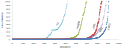
\includegraphics[width=8cm]{cdcl_comparison}
\caption{Die Laufzeitverteilung eines modernen CDCL SAT Solvers ohne Clause Learning, ohne VSIDS, ohne 2WL, ohne Restarts und mit allen Features eingeschaltet auf einem Benchmark aus 1000 SAT Problem Instanzen ~\cite{anatomy_of_modern_sat_solvers}}
\label{fig_sim}
\end{figure}

\subsection{SAT Competitions}
Abgesehen von einem direkten Vergleich auf einem divers gestalteten Benchmark aus vielen Problem Instanzen ist die Performance von SAT Solvern allgemein nur schwer zu vergleichen. Die Benchmarks der SAT 2018 Competition beinhalteten beispielsweise ein Problem mit mehr als 2,8 Millionen Variablen und über 11 Millionen Klauseln, welches in weniger als einer Stunde von MiniSat gelöst wurde, während ein anderes Problem mit nur 605 Variablen und 3664 Klauseln nicht in der Zeit durch MiniSat lösbar war \cite{sat_2018_proceedings}.

Die SAT Competitions sind regelmäßige Veranstaltungen, bei denen aktuelle SAT Solver öffentlich miteinander verglichen werden. Sie lösen das Problem der Vergleichbarkeit von SAT Solvern durch die Bereitstellung einer großen Menge an Benchmarks und einer Plattform, auf der regelmäßig die besten SAT Solver auf diesen Benchmarks verglichen werden. Dadurch haben sie im Laufe der Jahre erheblich zur Entwicklung moderner SAT Solver beigetragen. \cite{the_international_sat_competitions}

% Zudem haben verschiedene Solver unterschiedliche Stärken und Schwächen, wie beispielsweise eine Präferenz für SAT, beziehungsweise UNSAT. Das ist schon allein daran erkennbar, dass es bei SAT Competitions gesonderte Ranglisten für die Lösung von SAT und UNSAT Problemen gibt, bei denen oft unterschiedliche Solver an der Spitze stehen. % TODO: add citation (vlt. international sat competitions)

\subsection{Entwicklung im Zeitverlauf}
Bei der ersten \cite{the_international_sat_competitions} SAT Competition 1992 traten insgesamt 35 SAT Solver an. Die zu lösenden Benchmarks bestanden aus sechs einfachen SAT Problemen mit bis zu 120 Variablen und 510 Klauseln und sechs schwierigen Problemen mit bis zu 215 Variablen und 920 Klauseln. Zehn der angetretenen Solver lösten die einfachen Probleme in unter 25.000 Sekunden und nur sech Solver lösten die sechs schwierigen Probleme in unter 125.000 Sekunden. Das beste Ergebnis waren 268 Sekunden für die einfachen und 19.255 Sekunden für die schwierigen Probleme. \cite{competition_1992}

Dass selbst die schwierigen Probleme von damals mit heutigen Mitteln innerhalb von wenigen Sekunden zu lösen wären liegt auf der Hand, angesichts dessen, dass bei heutigen SAT Competitions Probleme in deutlich kürzerer Zeit gelöst werden, die bis zu 10.000 mal so groß sind, wie die damaligen \cite{sat_2018_proceedings}. Es stellt sich allerdings die Frage, ob diese Performance Entwicklung zum großen Teil an der Verbesserung der verfügbaren Hardware liegt oder ob die Entwicklung der SAT Solver selbst eine entscheidende Rolle gespielt hat.

Fichte et. al. \cite{time_leap_challenge} vergleichen SAT Solver von vor 20 Jahren mit modernen Solvern auf Hardware von 1999 und 2019. Sie kommen zu dem Ergebnis, dass die Weiterentwicklung der Algorithmen tatsächlich einen großen Einfluss auf die Performance der modernen Solver hat. In einem Vergleich, bei dem moderne Solver auf alter Hardware gegen alte Solver auf moderner Hardware antreten, sind die Ergebnisse im Durchschnitt fast gleich gut, mit einem kleinen Vorteil für die modernen Solver. \cite{time_leap_challenge}

Zusätzlich ist anzumerken, dass die wichtigste Optimierung für den DPLL Algorithmus, Conflict Driven Clause Learning bereits zwischen 1992 und 1999 entwickelt wurden und in den alten Solvern, die Fichte et. al. \cite{time_leap_challenge} verwenden, bereits implementiert war. Die größte algorithmische Performance Verbesserung für SAT Solver, die zwischen 1992 und heute passiert ist, wurde also bei dem Experiment gar nicht in Betracht gezogen.
Unter Betrachtung dieser Tatsache und den Ergebnissen des Experiments lässt sich folgern, dass sehr wahrscheinlich die Entwicklung der SAT Solver selbst seit der ersten SAT Competition 1992 eine größere Rolle in der Performance Verbesserung von SAT Solvern gespielt hat, als die Entwicklung der Hardware über den selben Zeitraum.

% \subsection{Vergleich zu anderen Problemen}

% \section{Probleme bei der Parallelisierung von SAT}

\section{Moderne SAT Solver in der Praxis}
Im folgenden soll eine Vorstellung von der praktischen Anwendbarkeit von modernen SAT Solvern gegeben werden. Verglichen mit vielen anderen $\mathcal{NP}$-vollständigen Problemen hat SAT eine lange Historie von großen, sowie inkrementellen Verbesserungen in seinen Algorithmen und deren Implementierungen. Das hat dazu geführt, dass moderne SAT Solver eine competetive Performance auch bei der Lösung vieler anderer schwerer Problemen gegenüber entsprechenden spezialisierten Algorithmen haben \cite{applying_sat_to_hard_problems}.

\subsection{Formale Verifikation}
Bounded Model Checking (BMC) auf Basis von SAT Solvern wurde erstmals 1998 als Technik zur formalen Verifikation von Mikrochip Schaltkreisen vorgestellt. BMC ermöglicht es, formal zu verifizieren, dass ein System bestimmte Eigenschaften erfüllt. In der Praxis werden so Bugs in Hardware Designs entdeckt und das korrekte Verhalten von neuen Prozessoren garantiert. Formale Verifikation wurde auch schon vor der Einführung von SAT basiertem BMC in der Hardware Entwicklung eingesetzt, BMC reduzierte allerdings die Dauer einer formalen Verifikation realer Systeme von Tagen auf Minuten. \cite{sat_solving_in_practice_2008}

Heute werden BMC und andere SAT basierte Techniken der formalen Verifikation weiterhin in der Hardware Entwicklung und zunehmend in der Entwicklung vieler sicherheitskritischer Sofware Systeme verwendet. Der seL4 Microkernel ist beispielsweise der schnellste existierende Microkernel und zugleich formal nachweisbar sicher gegen Hacker Angriffe \cite{seL4}.

\subsection{Dependency Solving}
Dependency Solving ist ein wichtiger Teil jedes Package Managers. Das Ziel ist, einen Upgrade Plan zu erstellen, der alle Schritte und benötigten Abhängigkeiten in der richtigen Reihenfolge beschreibt, um ein Packet zu installieren, zu updaten, etc. Das Dependency Solving Problem ist $\mathcal{NP}$-vollständig für viele Komponenten Modelle, wie das der Linux Distribution Debian. Es gibt unterschiedliche Ansätze dieses Problem zu lösen, aber einer, der in der Praxis erfolgreich verwendet wird, ist das Problem in SAT zu übersetzen und einen SAT Solver zu verwenden. Verbreitete Package Manager, die einen SAT Solver verwenden, sind der Eclipse Plugin Manager, DNF und Zyppy aus den Linux Distributionen von SUSE und RedHat, sowie optional Debians apt. \cite{dependency_solving}

\subsection{Machine Learning}
Der gemeinsame Einsatz von SAT Solvern und Machine Learning ist ein aktuelles Forschungsgebiet und verspricht einerseits bessere SAT Solver durch den Einsatz von Machine Learning Modellen zur Konfiguration von SAT Solvern. Andererseits soll mit Hilfe von SAT Solvern die Erkärbarkeit von Machine Learning Modellen verbessert werden, die mit wachsenden Modellen ein großes Problem darstellt. Neue, logikbasierte Machine Learning Modelle versprechen nachvollziehbare Erklärungen für ihre Ergebnisse. Praktisch wird an der Umsetzung solcher Modelle basierend auf modernen SAT Solvern geforscht. \cite{computing_with_sat_oracles}

\section{Fazit}
Als historisch erstes $\mathcal{NP}$-vollständiges Problem ist SAT von großer theoretischer Bedeutung. Zugleich haben moderne SAT Solver, vorangetrieben durch Anwendungen in der Hardware Entwicklung und die SAT Competitions, aufgrund ihrer hohen Performance große praktische Relevanz. SAT Solver haben sich seit Anfang der 90er Jahre enorm weiter entwickelt und algorithmische Verbesserungen erzielt, die sogar die Entwicklung von Computer Hardware im selben Zeitzaum übertrifft. Ermöglicht durch diesen Fortschritt bieten SAT Solver heute eine Möglichkeit, viele schwere, praxisrelevante Probleme effizient zu lösen, ohne spezialisierte Solver für einzelne Probleme zu entwickeln. Dabei werden die Eigenschaften von SAT als $\mathcal{NP}$-vollständigem Problem ausgenutzt.

In der Zukunft sollen die Vorteile von modernen SAT Solvern in immer mehr Domänen genutzt werden. Beispielsweise zur Implementierung neuartiger Machine Learning Modelle, die besser nachvollziehbare Ergebnisse als aktuelle Modelle versprechen.

% \section{Diskussion}
% Aufgrund der stagnierenden Entwicklung von Computer Hardware \cite{end_of_moore} ist zu vermuten, dass die Weiterentwicklung der SAT Solver selbst einen erheblich größeren Einfluss haben wird, sollte es in der Zukunft weitere große Performance Verbesserungen geben. Dies ist vor allem im Bereich der parallelen SAT Solver zu erwarten, aber auch für Sequentielle Solver ist anhand der regelmäßigen Verbesserungen bei den SAT Competitions kein unmittelbares Ende der Entwicklung in Sicht.


% Literaturverzeichnis
\addcontentsline{toc}{section}{Literatur}
\printbibliography

\end{document}
